\begin{enumerate}[label=\thesection.\arabic*.,ref=\thesection.\theenumi]
\numberwithin{equation}{enumi}
\item
Sketch the Polar Plot for
\begin{align}
G(s) = \frac{1}{(1+s)(1+2s)}
\end{align}
\\
\solution  Then the given open loop Transfer Function is
\begin{align}
G(s) = \frac{1}{(1+s)(1+2s)}
\end{align}

Now we have to substitute s=j$\omega$\\
\begin{align}
G(\j\omega) = \frac{1}{(1+\j\omega)(1+2\j\omega)} 
\end{align}
\item
Then find the Magnitude of the Transfer Function
\\
\solution
\begin{multline}
      |G(\j\omega)| = \frac{1}{\sqrt{(1+(\omega^2))(1+(2\omega)^2}}
\end{multline}\\
\item
Next find the Phase of Transfer Function\\
\solution
\begin{align}
    \angle G(\j\omega) = \angle G(\j\omega)_{num} - \angle G(\j\omega)_{den}
\end{align}
\begin{multline}
    \angle G(\j\omega) = -\tan^{-1}(\omega)-\tan^{-1}(2\omega)
\end{multline}
\item
Polar plot is drawn based on this magnitude and phase of transfer function\\
\solution\\
For $\omega$=0 
\begin{align}
    |G(\j\omega)| = 1\\
    \angle G(\j\omega) = 0
\end{align}
For w= $\infty$
\begin{align}
    |G(\j\omega)| = 0\\
    \angle G(\j\omega) = -\pi
\end{align}
Next Polar Plot is drawn by varying $\omega$ from 0 to $\infty$.\\
%\usepackage{graphicx}
\begin{figure}
    \centering
    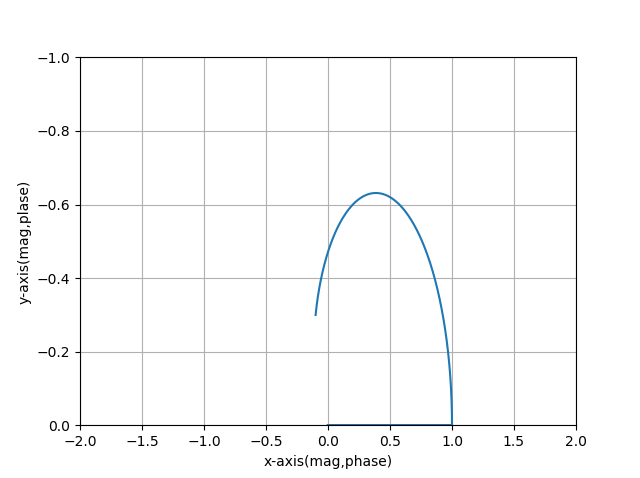
\includegraphics[width=0.7\linewidth]{ee18btech11012_1.png}
    \caption{Polar plot of given transfer function}
    \label{fig:Graph}
\end{figure}
\item
Verify the Polar Plot by running the following Code\\
\begin{lstlisting}
codes/ ee18btech11012_1.pyc
\end{lstlisting}
\item
What actually is a polar plot\\
The polar plot of the frequency response of a system is the line traced out as the frequency is changed from 0 to infinity by the tips of the phasors whose lengths represent the magnitude, i.e. amplitude gain, of the system and which are drawn at angles corresponding to their phase 
\item
Uses of Polar plots in control systems:\\
1.This is half of Nyquist plot running over positive frequencies.
\\
2.If we know type and order of a transfer function,we can easily draw its magnitude versus phase plot using polar plot.\\
For example,
In the given transfer function\\
\begin{align}
G(s) = \frac{1}{(1+s)(1+2s)}
\end{align}
Order is highest power of the polynomial in denominator of G(s),Type of system is number of poles at origin.\\
Here order=2,type=0\\
So this polar plot lies in third and fourth quardrant.
These order and type of a system determines shape of polar plot as shown in fig.4.7\\
\begin{figure}
    \centering
    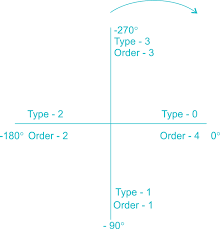
\includegraphics[width=0.7\linewidth]{ee18btech11012_4.png}
    \caption{Polar plot shape based on order and type}
    \label{fig:Graph}
\end{figure}
\item
Stability of transfer function\\
Polar plot also  determines stability of a system as\\
In the given transfer function\\
\begin{align}
G(s) = \frac{1}{(1+s)(1+2s)}
\end{align}
\\
Poles of G(s) are (-1,0),(-1/2,0) which lies on the left side of s-plane.

\\
As these poles (-1,0),(-1/2,0) are not encountered inside the polar plot as shown in fig.4.4.\\
The given transfer function G(s) is stable.






\end{enumerate}
